\section{Implementation and Experimental Results}
\label{sec:experimental} 

In this section, we describe our implementation of the three protocols
for privately computing edit distances between two strings and present
experimental results for network bandwidth and execution times.


We implemented the standard methods for secure circuit
evaluation, i.e., the Yao's ``garbled circuits'' method and secure computation
with shares.  We used the oblivious transfer protocol presented by Noar
and Pinkas~\cite{Naor-Pinkas:2001}.  For the min-of-3 computation, we used the lowest
price auction circuit of Kurosawa and Ogata~\cite{KO02}.
Using these primitives, we implemented the three protocols.  We also implemented the
protocol described by Atallah \textit{et al.}~\cite{atallah} for comparison, using the
efficient Lin-Tzeng \cite{lintzeng} millionaire's protocol, and Paillier~\cite{Paillier99}
homomorphic encryption. We used the
Fairplay compiler~\cite{Fairplay} to create circuits embedded in
the various protocols.  Fairplay converts a function
represented in a simple functional language into Boolean circuits.
We did not use the other functions of Fairplay, such as the actual secure circuit
evaluation protocol.

The experiments were executed on two 3-GHz Pentium 4 machines, with
two gigabytes of memory, and connected via a local LAN. Using this
setup, we obtained measurements (network bandwidth and execution
times) for the three protocols on various problem sizes. The reason
for performing the experiment on a local LAN is to provide a {}``best
case'' result for execution times in an environment where network
bandwidth is not a bottleneck. Because the bandwidth numbers presented
do not depend on the experimental setup, execution times for bandwidth-limited
networks can be estimated from the numbers presented here.

The size of the problem instance is $(n,m)$, where $n$ and $m$ are the
sizes of the two strings.  For simplicity, all experiments were performed
on problems where $m=n$.  The main conclusions that can be drawn from
our measurements are:

\begin{itemize}
\item {\it Protocol 1 is not suitable for large problems.} We observed that
the Fairplay compiler exhausted the two gigabytes of available memory on our
test machine while compiling a circuit for a problem instance of
size $(26,26)$. However, protocol 1 is ideal for small strings because the
entire computation is performed in one round.

\item {\it Protocol 2 can execute for problems of any size.}  It is a general
protocol that performs reasonably well for moderate size problems.  For example 
in our experimental
setup, a problem of size $(100,100)$ takes just under $9$ minutes.  Protocol 1
cannot scale to problems of this size.  For very small problems, Protocol 1 is more efficient.
Protocol 2 executes in $m+n-1$ rounds.

\item {\it Protocol 3 is most suitable for large problems.}
Protocol 3 uses the grid structure of the problem space, which makes
it most suitable for scaling up to larger problems. For example, a problem instance
of size $(200,200)$ takes under 10 minutes. Asymptotically, protocol 3
has the same performance as protocol 2, but since protocol 3 exploits
the grid structure of the problem space it is several times
faster.  Protocol 3 executes in $(m+n)/b-1$ rounds, where $b$
is the block size.

\item {\it The bandwidth requirements are asymmetrical.}  
This is primarily because Alice sends
the majority of data in the Naor-Pinkas~\cite{Naor-Pinkas:2001} oblivious transfer protocol.
This is useful if the parties are communicating using an asymmetrical network
connection, because the Alice's role can be assigned to the party with greater
bandwidth.

\item {\it The protocol by Atallah \textit{et al.}~\cite{atallah} is not efficient for practical use.}
It performed an order of magnitude worse than our secure circuit based protocols.  This is because
many large numbers (the homomorphic encrypted values) are computed and sent multiple times
 by both Alice and Bob at each step. For example, on problem instance of size $(25,25)$ the protocol
by Atallah \textit{et al.} took $5$ minutes and $35$ seconds. Protocol $3$ took $14$ seconds on the same problem
instance.
\end{itemize}

Figure~\ref{fig:histogram} shows the execution times for our three
protocols. Clearly, protocol $3$ scales the best as
the problem size increases. Protocol $1$ is suitable for small
problems. Protocol $2$ has a larger execution time, but only takes
limited bandwidth per round. Our experimental results confirm the
protocol characteristics discussed in Section~\ref{sec:protocols} (see
Figure~\ref{fig:protocol-characteristics}).

\begin{figure*}
\centering
%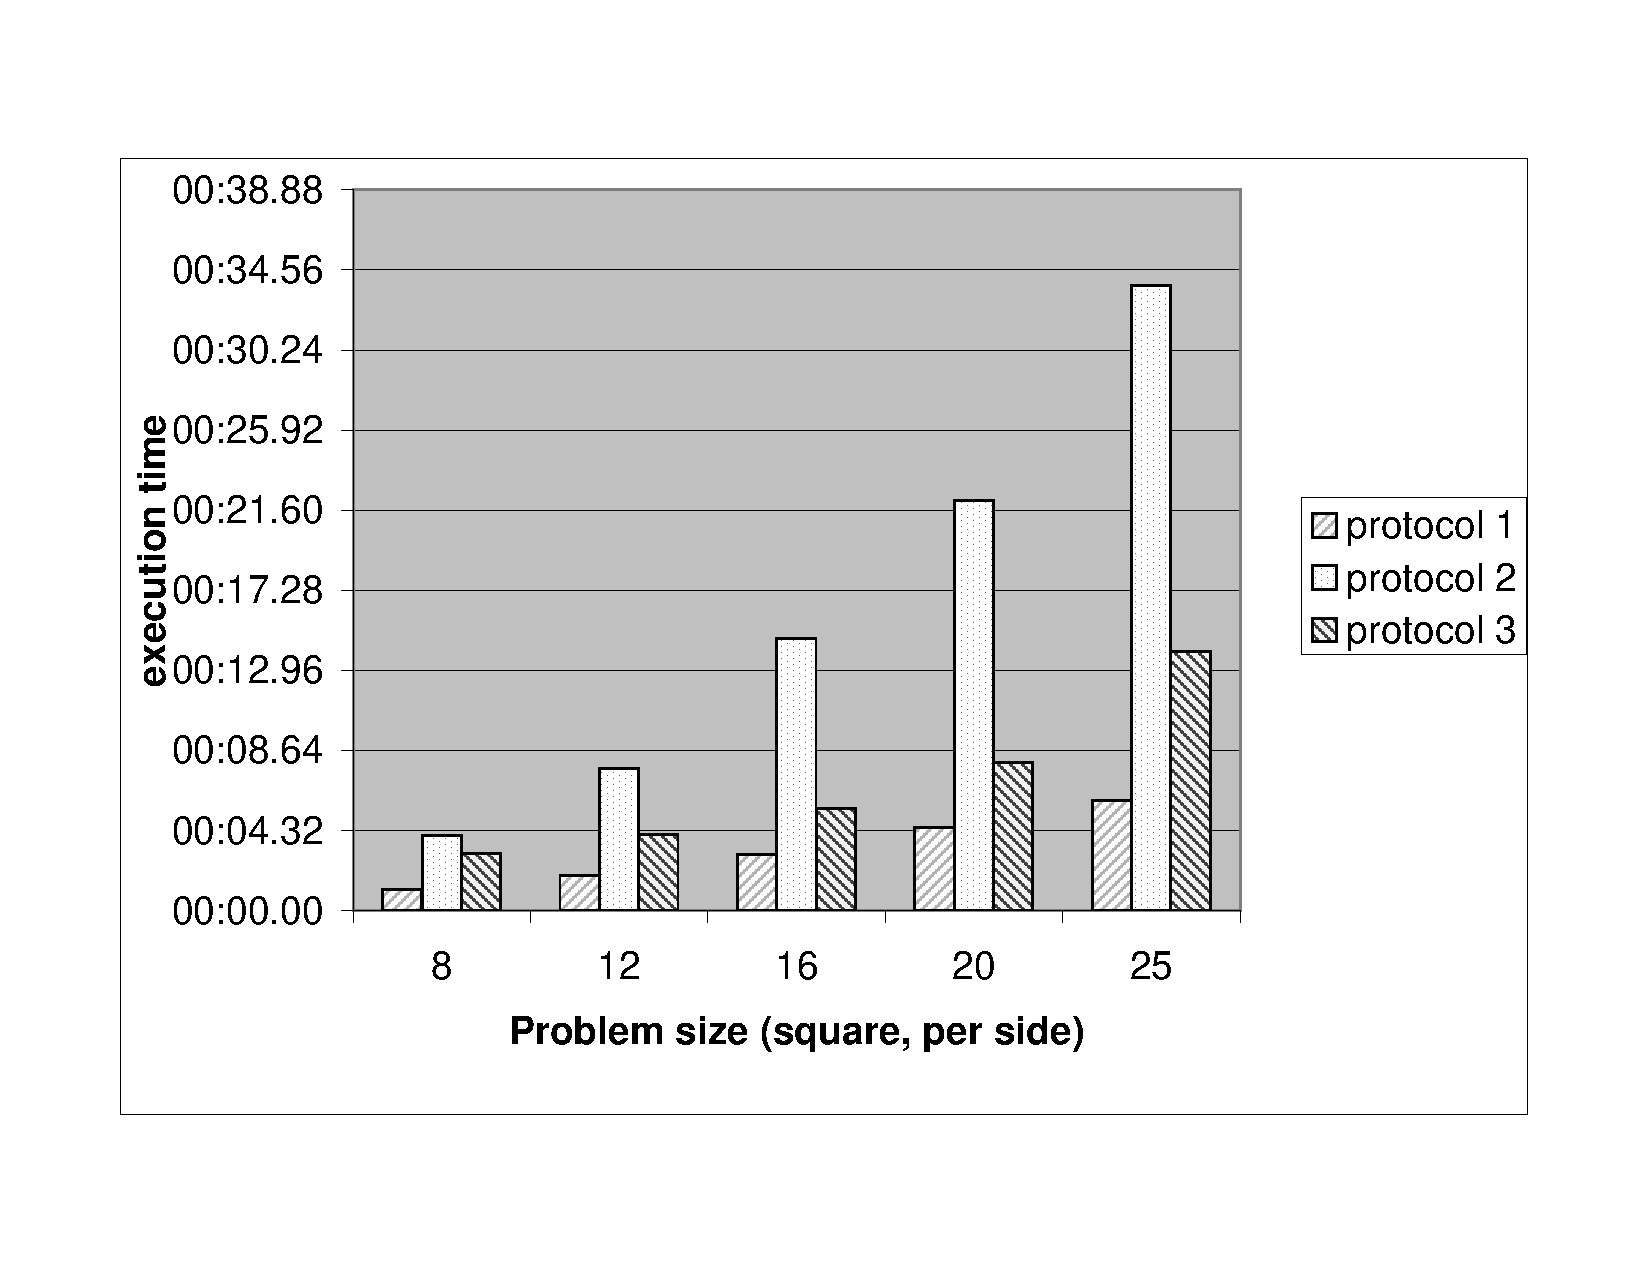
\includegraphics[bb=0bp 0bp 678bp 800bp,scale=0.5,angle=270]{figures/proto123}
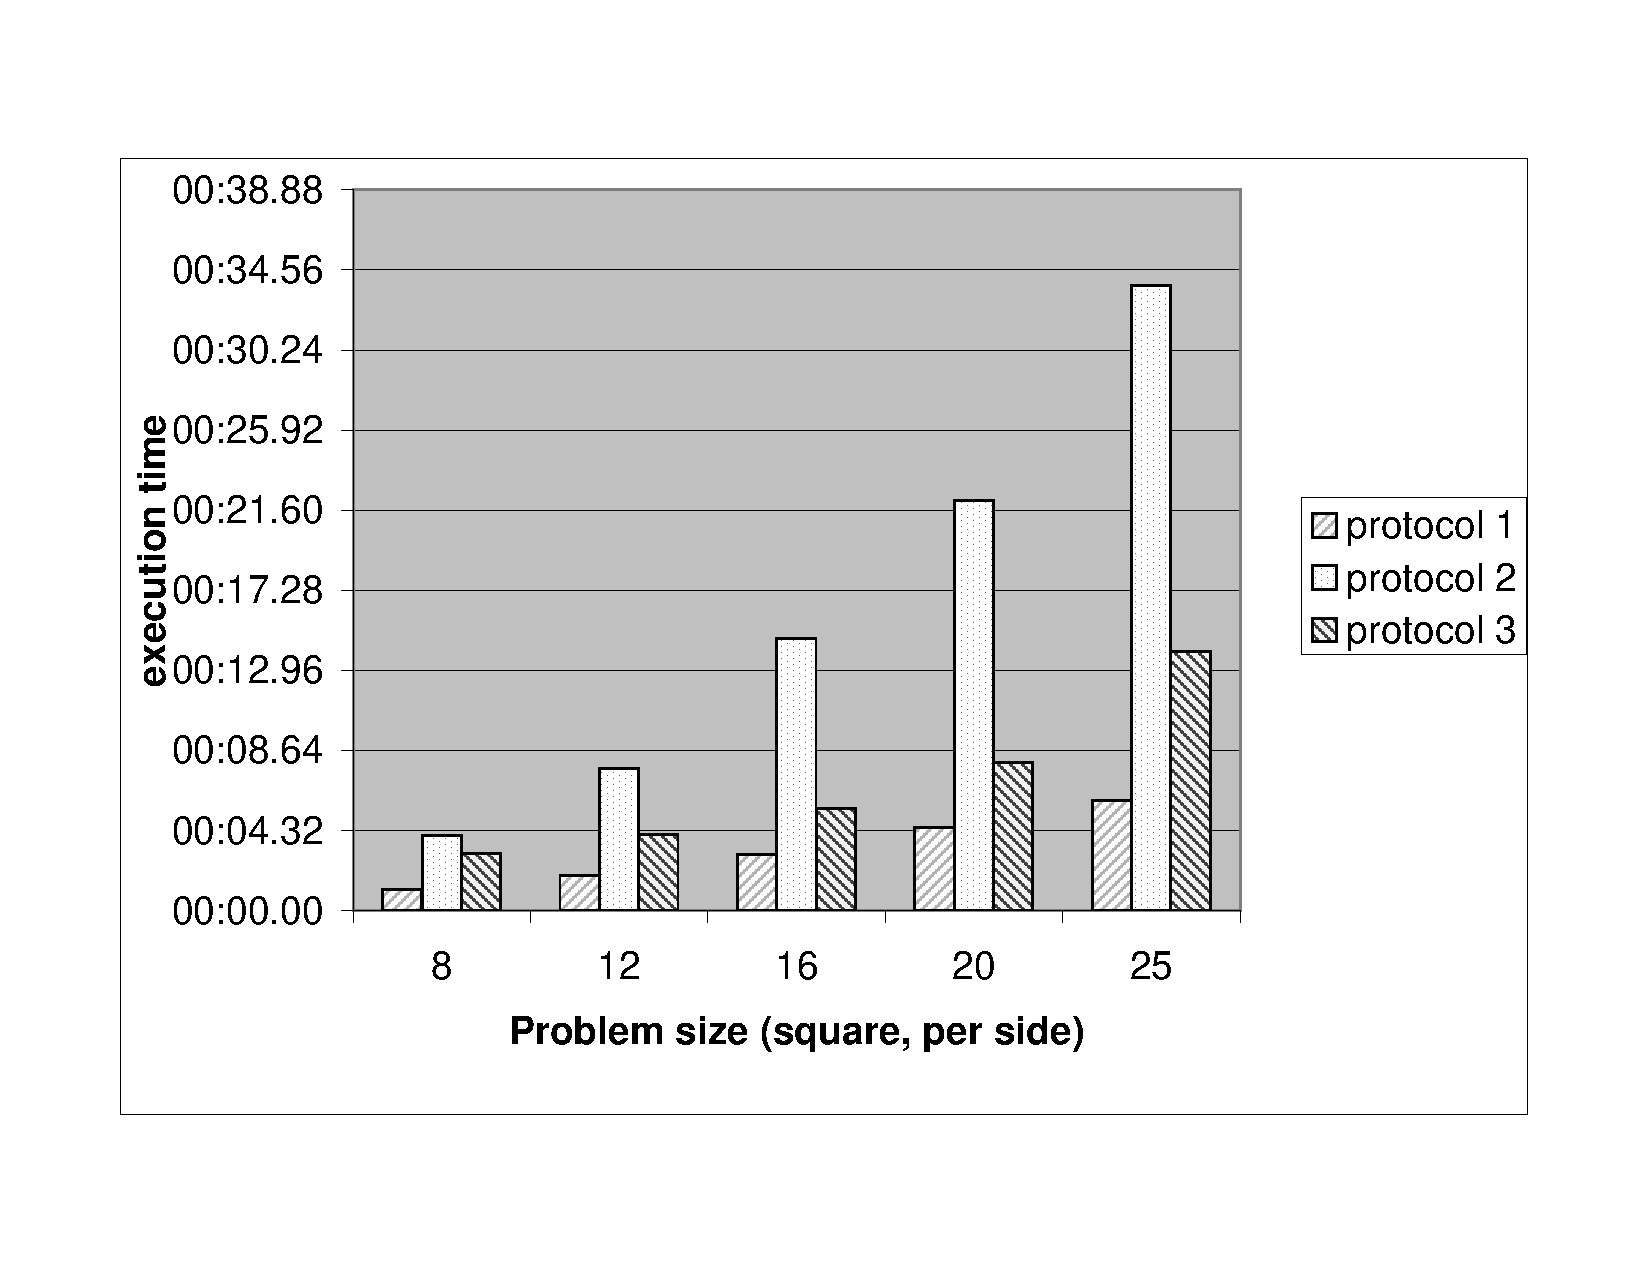
\includegraphics[scale=0.5,angle=270]{figures/proto123}

\caption{Timing measurements (in minutes and seconds) comparing protocols 1, 2, and 3.  For problem sizes (100,100) and (200,200), protocol 1 could not compile the circuit.}
\label{fig:histogram}
\end{figure*}

We present detailed results for protocols $1$ in the appendix. Results
for protocol $2$ can be found in Table~\ref{protocol2table}. We
discuss results for protocol $3$ in detail.  Recall that in this
protocol a grid is used (see the description in
Section~\ref{subsec:protocol3}). Using protocol $3$ we were able to
solve problems instances of considerable size. For protocol 3 we
present measurements for a problem instance of size
(200,200). Table~\ref{protocol3table200} shows the results using
various grid sizes. The performance steadily improves up to a grid size
of $20$, but the performance begins to slightly decrease after
that. However, continuing to increase the grid size slightly decreases
the network bandwidth requirement, which would result in fewer round
trips, so it would still be a consideration in environments with limited
network bandwidth. With a grid size of $20$, protocol 3 completes the
problem of size $(200,200)$ in just under the same amount of time as
protocol 2 takes for a problem of size ($25,25)$.
%Experimental results are visually shown in Figure~\ref{fig:proto3}.

%
\begin{table*}
\begin{center}
\begin{tabular}{|c||c|c|c|c|c|} \hline 
Problem size & Bandwidth (Alice) & Bandwidth (Bob) & CPU (Alice) & CPU (Bob) & wall clock \\ \hline \hline 
8x8 & 717 k & 68 k & 3.03 & 1.29 & 4.05 \\ \hline 
12x12 & 1.60 M & 154 k & 5.96 & 2.37 & 7.68 \\ \hline 
16x16 & 3.36 M & 315 k & 11.5 & 4.38 & 14.7 \\  \hline 
20x20 & 5.26 M & 492 k & 17.5 & 6.54 & 22.1 \\ \hline 
25x25 & 8.21 M & 769 k & 26.8 & 9.7 & 33.7 \\ \hline 
100x100 & 171.1 M& 32.0 M& 519 & 177 & 649 \\ \hline 
\end{tabular}
\end{center}

\caption{Network bandwidth (in bytes) and timing measurements (in seconds) for protocol 2 with
various problem sizes. (k and M are kilobytes and megabytes respectively)}
\label{protocol2table}
\end{table*}

\begin{table*}
\begin{center}
\begin{tabular}{|c||c|c|c|c|c|} \hline 
Grid size & Bandwidth (Alice) & Bandwidth (Bob) & CPU (Alice) & CPU (Bob) & wall clock \\ \hline \hline 
25 & 362.2 M & 2.1 M & 518 & 84 & 658 \\ \hline 
20 & 368.5 M & 2.6 M & 385 & 90 & 534 \\ \hline 
10 & 397.4 M & 5.4 M & 476 & 123 & 655 \\  \hline 
8 & 412.0 M & 5.8 M & 520 & 145 & 729 \\ \hline 
4 & 485.3 M & 14.4 M & 784 & 234 & 1095 \\ \hline 
2 & 635.2 M& 32.0 M& 1296 & 408 & 1804 \\ \hline 
1& 948.0 M& 76.7 M& 2480 & 780 & 4883 \\ \hline
\end{tabular}
\end{center}

\caption{Network bandwidth (in bytes) and timing measurements (in seconds) for protocol 3 with
a problem of size $(200,200)$. (M refers to Megabytes)}
\label{protocol3table200}
\end{table*}




%
%\begin{figure}
%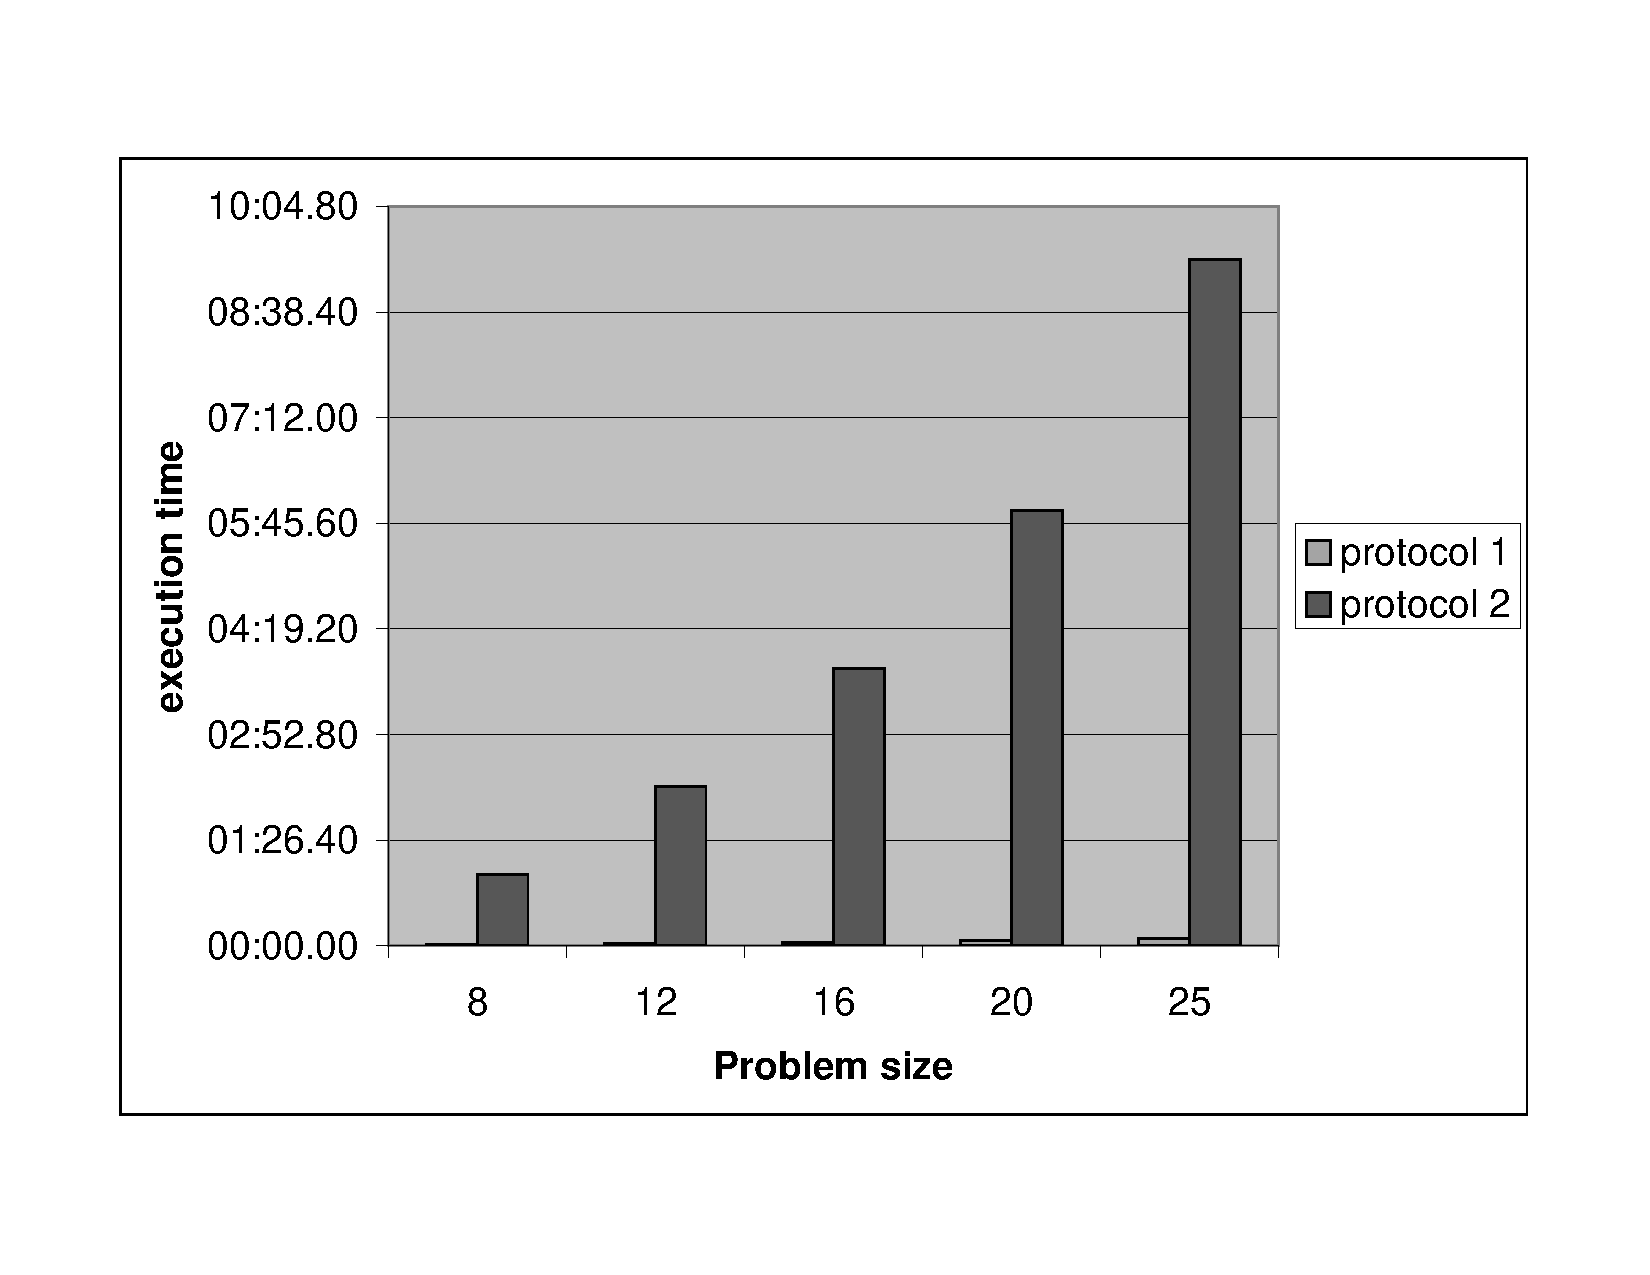
\includegraphics[bb=0bp 0bp 678bp 800bp,scale=0.5,angle=270]{figures/proto12}
%\caption{Comparison of execution time for protocols 1 and 2\label{fig:proto12}}
%\end{figure}


%
%\begin{figure}
%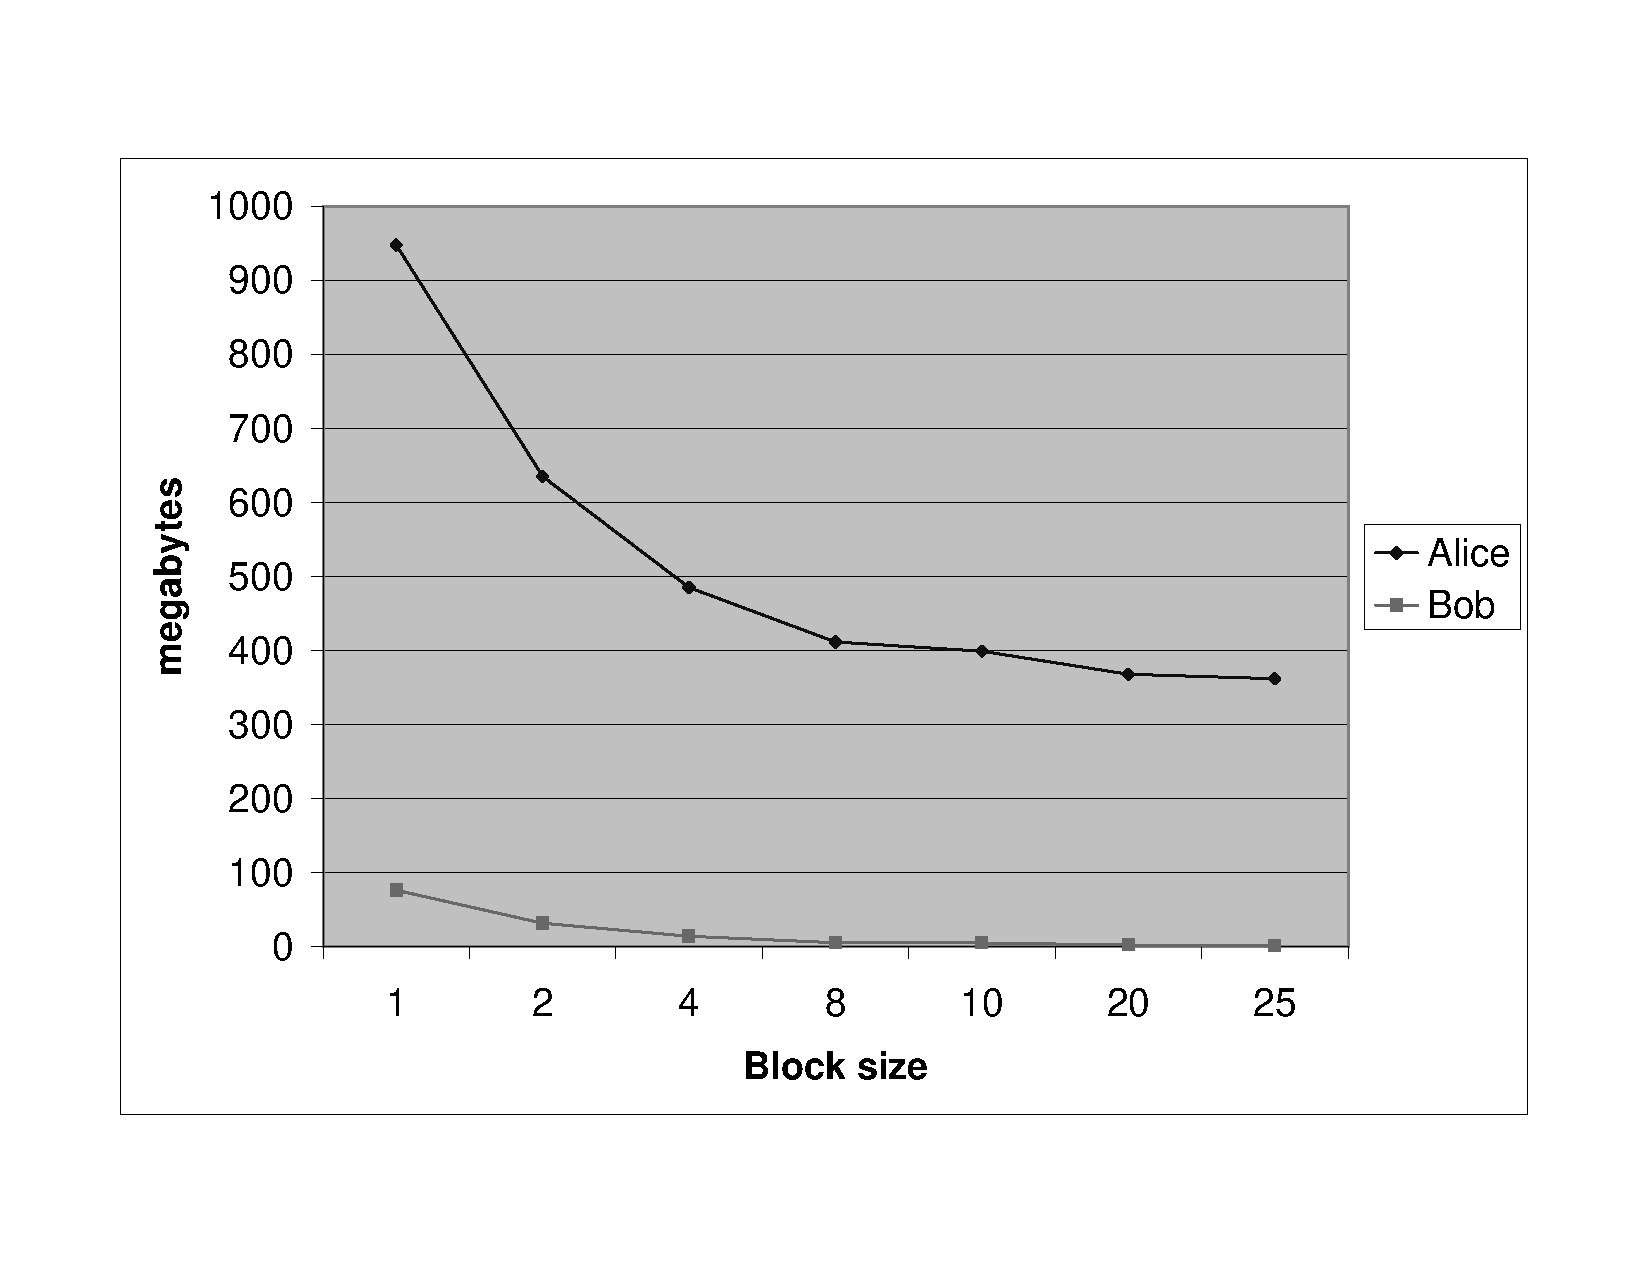
\includegraphics[bb=0bp 0bp 678bp 800bp,scale=0.3,angle=270]{figures/p3bytes}
%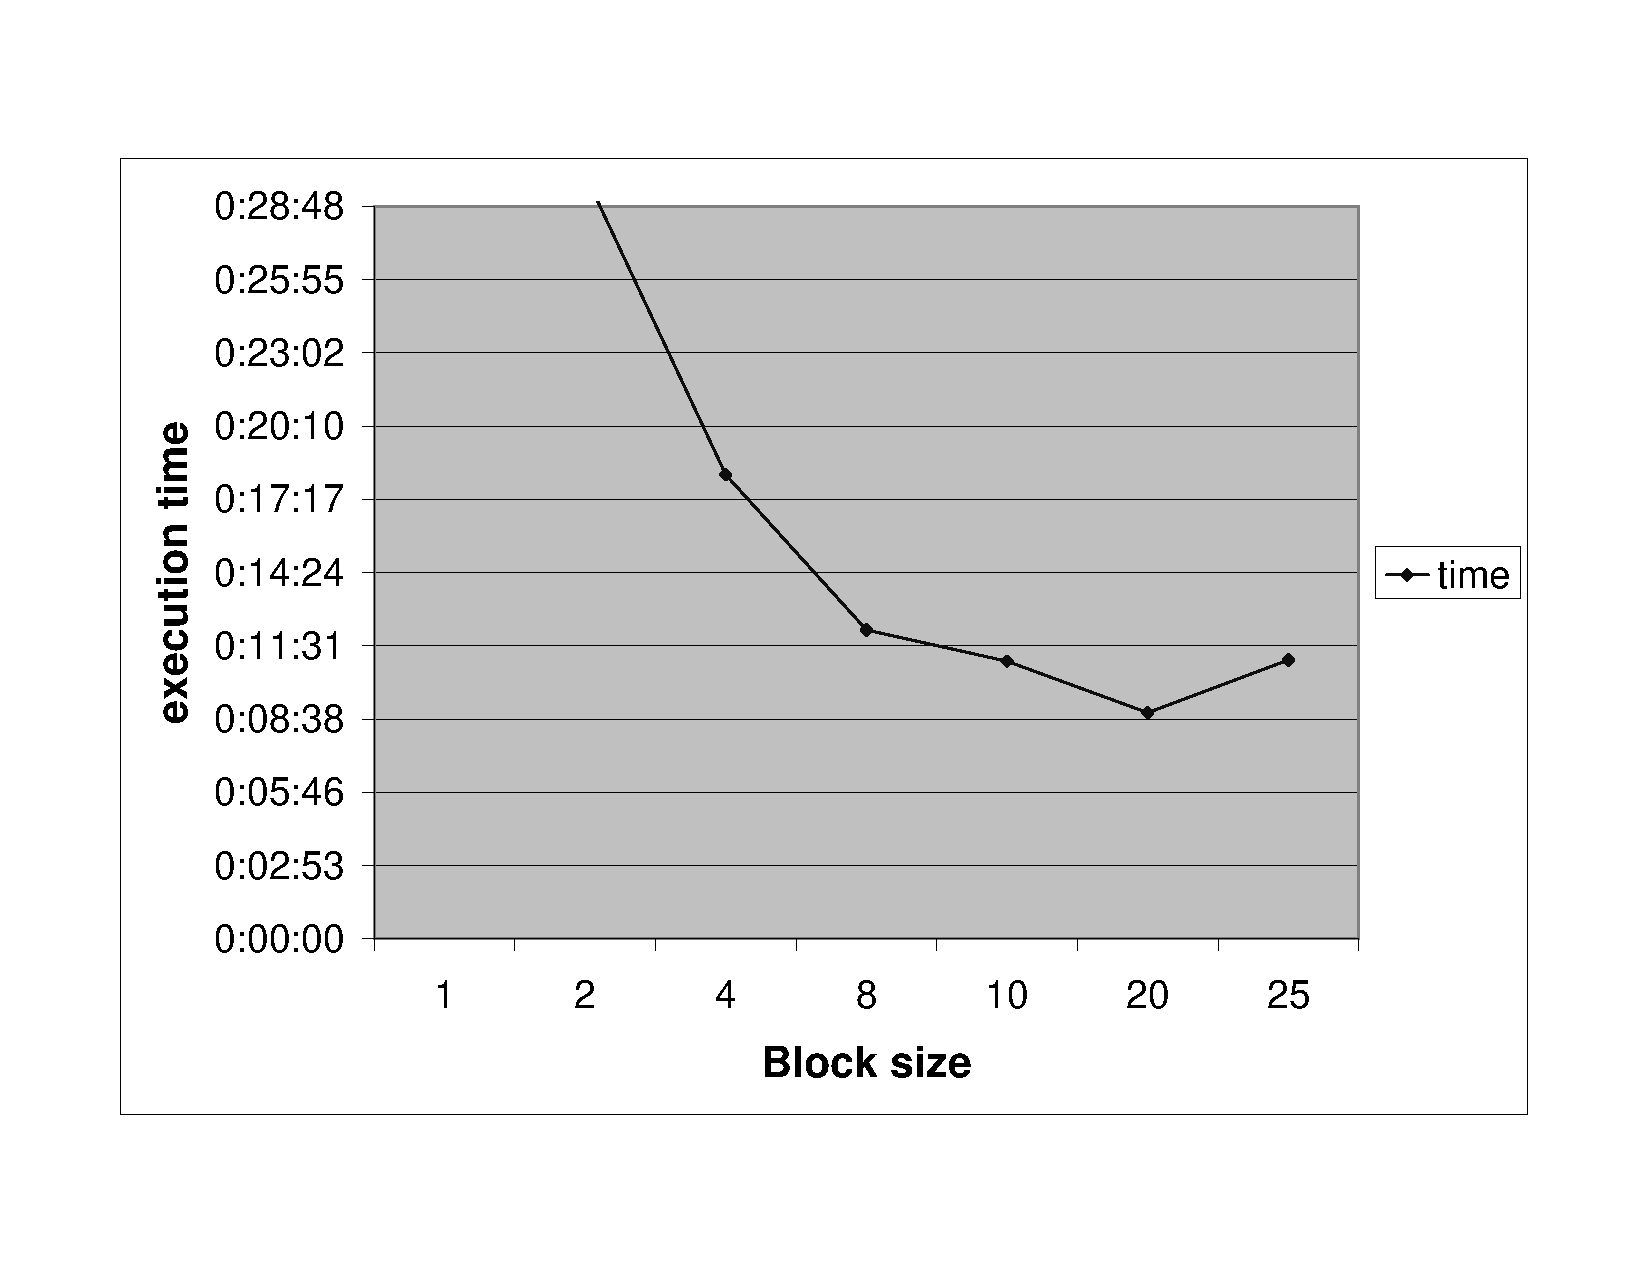
\includegraphics[bb=0bp 0bp 678bp 800bp,scale=0.3,angle=270]{figures/p3time}


%\caption{Network and timing measurements of a 200x200 problem using protocol 3\label{fig:proto3}}
%\end{figure}

